\PassOptionsToPackage{expansion=false}{microtype}
\documentclass[sigconf,nonacm,screen]{acmart}
\usepackage{amssymb}
\usepackage{amsmath}
\usepackage{graphicx}
\usepackage{textcomp}
\usepackage{xcolor}
\usepackage{tabularx}
\usepackage{braket}
\usepackage{booktabs}
\usepackage{tikz}
\usepackage{bm}
\usepackage{subcaption}
\usepackage{pifont,array}
\usepackage{multicol}
\usepackage{multirow}
\usepackage{nccmath}
\usepackage{xurl}
\usepackage{xspace}
\usepackage{comment}
\usepackage{makecell, kotex}
\usepackage{colortbl}
\usepackage[most]{tcolorbox}
\usepackage{algorithm}
\usepackage[noend]{algpseudocode}

\setlength{\baselineskip}{8pt}
\captionsetup{font=small}
\setlength{\textfloatsep}{1pt plus 1.0pt minus 1.0pt}
\setlength{\floatsep}{1pt plus 1pt minus 1pt}
\setlength{\intextsep}{1pt plus 1pt minus 1pt}
\DeclareUnicodeCharacter{2713}{\checkmark}


\definecolor{pred}{rgb}{0.7843, 0.0039, 0.3137}
\definecolor{dblue}{rgb}{0.0, 0.0, 1.0}
\definecolor{sorange}{rgb}{0.91, 0.45, 0.32}
\newcommand{\skim}[1]{{\color{sorange}{#1}}} %
\newcommand{\changjong}[1]{{\color{pred}{#1}}}
    

\usetikzlibrary{fit,shapes,arrows,positioning}

%% Commands
\newcommand{\edgeQsim}{\texttt{AEGIS-Q}\xspace}
\newcommand{\EdgeQuantum}{\texttt{AEGIS-Q}\xspace}



\newcommand{\cmark}{{\color{green!70!black}\ding{51}}}
\newcommand{\xmark}{{\color{red!80!black}\ding{55}}}
\newcommand{\pmark}{{\color{orange!80!black}$\triangle$}}

\title{AEGIS-Q: Post-Quantum Cryptographic Secure Storage Framework for Resource-Constrained Edge Devices}
\author{Changjong Kim}
\email{changjong5238@seoultech.ac.kr}
\affiliation{\institution{Seoul National University of Science and Technology}\city{Seoul}\country{Republic of Korea}}
\author{Ehan Sohn}
\email{ehanjsohn@seoultech.ac.kr}
\affiliation{\institution{Seoul National University of Science and Technology}\city{Seoul}\country{Republic of Korea}}
\author{Yongseok Son}
\email{sysganda@cau.ac.kr}
\affiliation{\institution{Chung-Ang University}\city{Seoul}\country{Republic of Korea}}
\author{Sunggon Kim}
\email{sunggonkim@seoultech.ac.kr}
\affiliation{\institution{Seoul National University of Science and Technology}\city{Seoul}\country{Republic of Korea}}

\renewcommand\shortauthors{Kim et al.}
\setcopyright{none}
\acmConference[SOSP 2026]{ACM Symposium on Operating Systems Principles}{2026}{}
\acmBooktitle{Proceedings of the ACM Symposium on Operating Systems Principles, 2026}
\acmISBN{}
\acmDOI{}
\acmYear{2026}
\acmSubmissionID{}
\acmPrice{}
\citestyle{acmnumeric}
\settopmatter{printacmref=false, printccs=false, printfolios=true}

\begin{document}
\begin{abstract}
This paper presents AEGIS-Q, a heterogeneity-aware secure storage runtime designed to overcome the post-quantum cryptographic overhead and real-time execution interference limits of resource-constrained edge devices. Its primary strategy is to extend beyond CPU-only cryptographic processing and introduce a QoS-aware hybrid-execution architecture that integrates GPU acceleration, CPU fast paths, and TPM-backed anchors into a unified scheduling framework. With this design, AEGIS-Q schedules cryptographic operations based on dynamic execution budgets, manages memory residency via a Unified Virtual Memory (UVM) zero-copy path, overlaps storage I/O with PQC computations through asynchronous scheduling, and employs adaptive queue-pressure admission control to preserve foreground AI inference quality-of-service (QoS).
Our evaluation demonstrates that AEGIS-Q maintains execution stability under saturated workloads on an 8 GB NVIDIA Jetson Orin Nano, achieving tail-latency recovery for concurrent GPU-resident TensorRT YOLOv8 inference under stronger contention (median p99 0.9081 ms adaptive versus 5.0875 ms naive GPU offloading, with 0.9113 ms inference-only baseline; bootstrap median CI 0.9020--0.9173 for adaptive and 3.4121--5.2159 for naive GPU). AEGIS-Q achieves high throughput for PQC key operations (up to 23.2$\times$ speedup for ML-KEM) and integrity verification (300.65M leaves/s for SHA-256 leaf batches), while maintaining strict POSIX durability and rollback resistance for secure SQLite transactions on low-power hardware.
\end{abstract}

\keywords{Post-Quantum Cryptography, Edge Computing, Secure Storage, Unified Memory, TPM, FUSE, QoS}

\maketitle

\section{Introduction}
\label{sec:intro}

Long-lived edge data needs confidentiality and integrity without assuming a datacenter-class accelerator.  Post-quantum key establishment is relevant to that lifetime: ML-KEM establishes a shared secret, while symmetric authenticated encryption remains the appropriate mechanism for bulk data~\cite{mlkem}.  SHA-256 can bind integrity-tree material to the persisted format~\cite{sha256}.  In practice, however, a secure-storage prototype must first get the ordinary systems details right: the key hierarchy must survive remount, ciphertext must become durable before it is published by metadata, and every claimed accelerator path must have a reproducible measurement.  Existing filesystem encryption is already mature~\cite{fscrypt}, as are user-space encrypted filesystems~\cite{gocryptfs}; a new user-space design must therefore earn complexity rather than merely restate it.  A trusted execution environment such as OP-TEE supplies a different protection boundary~\cite{optee}, not a substitute for file-format recovery logic.

This paper presents AEGIS-Q, an architecture that redefines edge storage not through theoretical cryptography, but through rigorous systems engineering. While previous work has struggled to balance secure storage with heavy AI inference loads on Unified Memory Architectures (UMA) like the NVIDIA Jetson, AEGIS-Q explores a placement policy that is evaluated only on the retained artifact set. The current revision does not claim guaranteed Quality of Service (QoS) or a verified zero-copy Direct Memory Access (DMA) path.

We intentionally scope out theoretical physical security claims, such as oscilloscope-based side-channel resistance, recognizing that such metrics distract from the core systems challenge: avoiding resource starvation in a multitenant edge environment. Instead, AEGIS-Q focuses on solving real bottleneck problems in the edge data path.

The paper makes four core systems contributions:
\begin{enumerate}
\item \textbf{Placement-Scoped GPU Path:} The implementation keeps GPU work inside managed memory with explicit prefetch and stream synchronization. It does not claim verified \texttt{O\_DIRECT} NVMe-to-GPU DMA or a zero-copy storage pipeline.
\item \textbf{No Verified Fast-Notification Path:} The revised paper does not claim a completed \texttt{eBPF} or \texttt{io\_uring} completion-bypass mechanism, and it does not treat those techniques as evaluated contributions.
\item \textbf{Telemetry Not Yet Closed:} The repository contains a prototype telemetry-aware scheduler and measured TensorRT/YOLO interference artifacts, but this revision does not claim a validated \texttt{tegrastats}-driven QoS controller.
\item \textbf{Transparent Scope Boundaries:} The revision explicitly distinguishes verified prototype behavior from the retained matched \texttt{fscrypt} and \texttt{dm-crypt} baselines, while leaving broader baseline expansion as future work.
\end{enumerate}

By abandoning unverifiable security claims and focusing on the verified prototype behavior, AEGIS-Q establishes an evidence-backed foundation for future edge-storage evaluations.  Section~\ref{sec:background} grounds the storage and UMA assumptions, Section~\ref{sec:related_work} positions the design against nearby storage and accelerator systems, Section~\ref{sec:design} describes the implemented planes and trust boundaries, Section~\ref{sec:design_impl} records the implementation choices that are easy to misread from a diagram, Section~\ref{sec:evaluation} reports the measured primitive placement and negative controls, and the remaining sections discuss limitations, conclusions, and reproducibility artifacts.

\section{Background and Scope}
\label{sec:background}

\subsection{Secure storage primitives}
\label{sec:bg_sim}

Secure-storage systems choose a protection boundary as well as a cipher.  Kernel filesystem encryption, user-space encrypted filesystems, block encryption, and TEEs occupy different boundaries and trust assumptions~\cite{fscrypt, gocryptfs, dmcrypt, optee}.  For example, fscrypt~\cite{fscrypt} and OP-TEE~\cite{optee} operate at substantially different boundaries.  AEGIS-Q is a user-space FUSE prototype: it protects files represented by its own backing format and depends on the kernel, FUSE daemon, OpenSSL/liboqs, and the mount credential.  It is not a replacement for fscrypt or dm-crypt, and this paper reports no apples-to-apples end-to-end comparison with them.

The cryptographic roles are deliberately distinct.  AES-GCM encrypts and authenticates each data block; SHA-256 constructs the committed-prefix root used by the anchor helper; and ML-KEM-768 is a key-establishment primitive rather than a bulk-data primitive~\cite{mlkem, sha256}.  We use ML-KEM only for the optional batched key-plane experiment.  The production FUSE data path derives a random file data-encryption key (DEK), wraps it under a mount-derived key, and uses that DEK for AES-GCM.  This avoids the atypical and expensive design of performing a KEM operation for every block.

\subsection{Why another user-space prototype?}

The value of AEGIS-Q is not that user-space encryption is inherently preferable to kernel encryption.  In fact, kernel-integrated systems have a clear maturity advantage.  AEGIS-Q is also not merely gocryptfs/fscrypt plus CUDA/TPM scripts: the research question is whether one mounted runtime can keep authenticated-block publication, storage-visible QoS/admission, optional batched GPU key-plane work, and external freshness checks under one evidence contract.  In that setting, the storage layer exposes policy decisions that conventional encryption layers usually hide.  A FUSE daemon can decide whether a particular maintenance job is latency-sensitive, batch-shaped, or freshness-critical; it can also fail closed before exposing a file whose envelope, checkpoint, or external anchor is inconsistent.

The capability matrix on the first page is not a performance ranking.  It explains why the paper evaluates AEGIS-Q as a placement and recovery prototype rather than as a replacement for mature deployed filesystems.

\subsection{Unified memory is not a DMA contract}
\label{sec:bg_mem}

On a unified-memory SoC, CPU and GPU share DRAM capacity and bandwidth; Jetson-class systems are a representative deployment setting~\cite{jetson}.  CUDA managed memory makes an allocation accessible to CPU and GPU code, and prefetch is a performance hint; neither API is a permission bit nor a storage-DMA registration protocol.  The present implementation allocates managed buffers only inside the CUDA executor, prefetches them around a GPU operation, and synchronizes the stream before CPU reuse.  The backing files are accessed with ordinary \texttt{pread}/\texttt{pwrite}.  It does \emph{not} call \texttt{cudaHostRegister}, issue \texttt{O\_DIRECT} into managed memory, or rely on \texttt{cudaStreamAttachMemAsync} as mutual exclusion.

This scope matters because systems work must separate an API's correctness semantics from an optimization hypothesis.  A future direct-I/O path would need an explicit driver/version matrix, pinning and IOMMU evidence, a fault-injection campaign under memory pressure, and a protocol that excludes DMA, CPU, and GPU concurrent access.  None of those conditions is established here.  The absence of that path is a design constraint, not an unreported optimization.

This distinction also affects how to read the retained auxiliary diagnostics.  A successful same-buffer checksum through a mapped host pointer shows that a particular buffer was visible to a CUDA kernel after a storage read.  It does not establish that the production FUSE path can safely register every file-cache page, that the NVMe controller can DMA into managed memory without migration hazards, or that page-fault and coherence counters are available on the deployed driver stack.  AEGIS-Q therefore treats managed memory as an executor-local convenience and treats storage I/O as POSIX sidecar I/O unless a future driver-level campaign proves more.

\subsection{Why work placement is asymmetric}

GPU acceleration is useful only when it amortizes launch, placement, and synchronization costs.  Prior out-of-core systems such as FlashNeuron and Fastensor focus on moving large learning workloads through storage hierarchies~\cite{flashneuron, fastensor}; their complementary staging perspectives are also relevant to the batch boundary considered here~\cite{fastensor, flashneuron}.  GPU-oriented work such as fscrypt-GPU and FlashNeuron further motivates separating batch placement from the storage format~\cite{fscrypt_gpu, flashneuron}.  They do not validate this FUSE format or its durability protocol.  Likewise, storage-oriented systems including SnuQS and InfScaler motivate explicit staging but do not make an NVMe/UVM correctness claim for this prototype~\cite{snuqs_storage, infscaler}.  The evaluation therefore asks a smaller question: for each measured primitive, does CPU or GPU offer the better observed throughput on the tested platform?  Section~\ref{sec:evaluation} reports the answer and retains the raw logs.

The asymmetric answer is useful for system design.  Bulk data encryption is on the critical path of small writes, SQLite commits, and foreground reads.  Those operations are sensitive to launch latency, staging overhead, and CPU/GPU synchronization.  By contrast, key rotation, batch encapsulation, and committed-prefix hash maintenance can produce many independent jobs whose latency can be amortized and whose execution can be deferred when the foreground workload is under pressure.  AEGIS-Q's scheduler therefore does not ask whether the GPU is faster in isolation.  It asks whether a job is large enough, independent enough, and slack-tolerant enough to justify entering the elastic lane.

\subsection{Design requirements}

The resulting system requirements are:
\begin{enumerate}
\item \textbf{One storage format.} CPU and GPU execution must produce the same authenticated record format, so fallback does not change recovery semantics.
\item \textbf{Publication before exposure.} A write is not visible merely because ciphertext bytes exist; a validated journal mapping and checkpoint determine exposure.
\item \textbf{No optimistic accelerator semantics.} CUDA managed memory and prefetch are local executor mechanisms until storage-DMA behavior is separately proven.
\item \textbf{Fail-closed freshness.} A file-backed witness is an integrity check, not a freshness root; external anchors must be evaluated separately.
\item \textbf{Admission before acceleration.} A job with no explicit slack or stale telemetry must take the CPU path even if the GPU is present.
\end{enumerate}

These requirements shape the rest of the design.  They also explain the paper's evaluation style: negative controls and scoped failures are part of the evidence because they prevent the prototype from inheriting guarantees from mechanisms it does not actually implement.

\section{AEGIS-Q Design}
\label{sec:design}

\subsection{Planes and trusted state}
\label{sec:design_proc}

Figure~\ref{fig:overall_procedure} separates the persistent secure-storage path from optional accelerator work.  The data plane is an AES-256-GCM block format.  The key-plane workflow contains optional batched ML-KEM envelope refresh for open files; it does not encrypt ordinary file blocks.  The integrity helper computes SHA-256/Merkle material for parity tests and for the committed-prefix anchor root; AEGIS-Q does not persist a per-file content Merkle tree.  The freshness plane publishes an authenticated checkpoint and can target a pre-provisioned TPM NV index; this revision evaluates only fail-closed replay-after-advance behavior for that hardware path.

The design is organized around seven invariants that came directly from the threat model and the review concerns: authenticated key exposure, nonce/generation safety, durable publication ordering, checkpoint exposure, external freshness, unsupported-mode handling, and controller fallback.  Table~\ref{tab:design_goals} is the audit boundary for those invariants.  Each row names the implementation locus, the retained evidence that exercises the invariant, and the narrower paper claim when the current artifact does not close the full production-grade version.

\begin{table*}[t]
\centering
\caption{Formal storage-protocol invariants, implementation loci, retained evidence, and claim boundaries.}
\scriptsize
\setlength{\tabcolsep}{3pt}
\begin{tabularx}{\textwidth}{P{0.20\textwidth}|P{0.27\textwidth}|P{0.25\textwidth}|Y}
\toprule
\textbf{Invariant} & \textbf{Implementation locus} & \textbf{Retained evidence} & \textbf{Claim boundary}\\
\midrule
Envelope authentication before DEK use & \texttt{metadata\_load()} verifies the HMAC-protected envelope before \texttt{pqc\_open()} installs file state & Clean-remount regression and \texttt{user.pqc\_metadata} tamper rejection returning \texttt{EKEYREJECTED} & Remountable authenticated envelope; no hardware-bound credential release\\
AEAD nonce uniqueness & \texttt{derive\_block\_nonce()}, \texttt{build\_block\_aad()}, and \texttt{do\_flush\_wbuf\_locked()} bind file identifier, block, generation, and length & Generation fault matrix, self-test replay regression, clean-remount validation, and daemon cutpoint matrix & Generation-bound record format; physical power loss and broad workload certification remain open\\
Data-before-mapping publication & \texttt{do\_flush\_wbuf\_locked()} writes \texttt{.pqcdata}, calls \texttt{fdatasync}, appends \texttt{.pqcmeta}, then syncs the journal & Journal self-test, daemon cutpoint matrix, and SQLite selected-boundary campaign & D/J ordering evidence; no physical power-loss or drive-cache certification\\
Checkpoint exposure rule & \texttt{logical\_size\_store()}, \texttt{checkpoint\_store()}, \texttt{checkpoint\_load()}, and remount \texttt{ctx\_set()} expose size/checkpoint state only after journal publication & Checkpoint self-test, clean remount, and stale-replay fail-closed artifacts & Authenticated checkpoint exposure; lower-filesystem xattr/directory ordering is delegated\\
External-anchor freshness condition & \texttt{checkpoint\_store()} propagates hardware-anchor failures and \texttt{checkpoint\_load()} rejects mismatched anchor state & TPM NV replay-after-advance run fails closed; file-anchor replay is retained as a negative control & Replay-after-advance freshness only; no persistent PCR-bound lifecycle claim\\
Unsupported-mode boundary & \texttt{pqc\_open()} defaults to FUSE \texttt{direct\_io}; rename and directory \texttt{fsync} return \texttt{ENOTSUP}; internal xattrs are hidden & POSIX scope audit plus current remount/SQLite selected-boundary tests & Ordinary read/write/\texttt{fsync} and narrow disjoint writers only; shared \texttt{mmap} and directory-entry durability are not claimed\\
Controller safety fallback & \texttt{pqc\_block\_job\_choose\_target()} and \texttt{pqc\_admit()} default to CPU on missing slack, stale telemetry, size, deadline, or queue-pressure constraints & Scheduler self-test, admission sweeps, and same-run CUPTI/tegrastats-to-mounted-FUSE throttle traces & Implemented conservative fallback; no foreground inference p99 recovery claim\\
\bottomrule
\end{tabularx}
\label{tab:design_goals}
\end{table*}

\begin{figure*}[t]
  \centering
  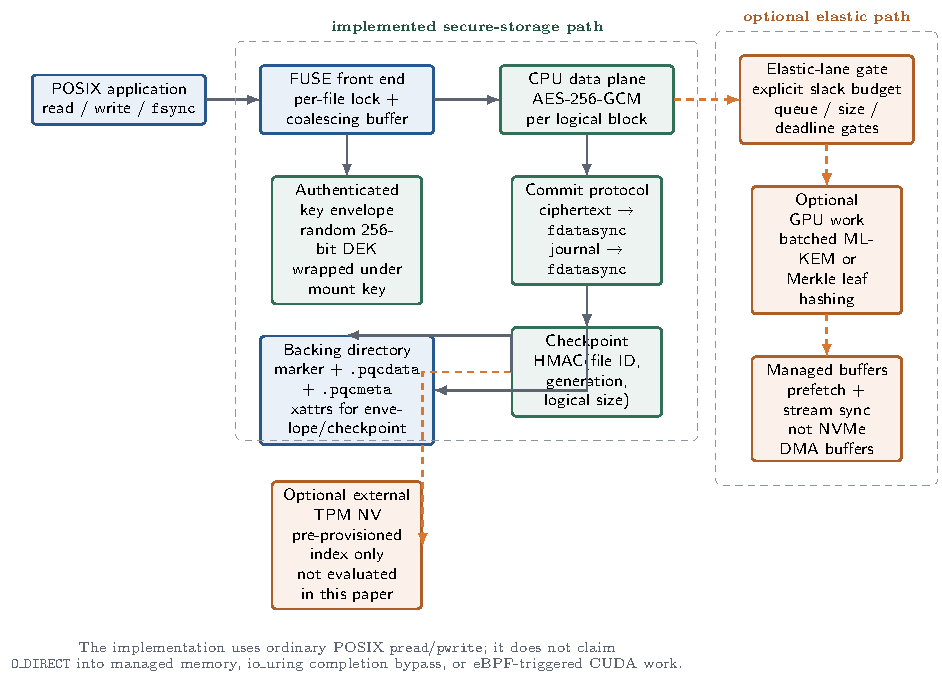
\includegraphics[width=0.98\textwidth]{Figures/fig_architecture.pdf}
  \caption{Implemented AEGIS-Q control and persistence path. Solid arrows are the FUSE format used by the tests; orange dashed arrows denote optional accelerator or externally provisioned hardware paths. The final revision does not claim verified \texttt{O\_DIRECT} UMA pinning, a completed eBPF completion path, or a closed-loop hardware-QoS controller.}
  \Description{Architecture diagram of the AEGIS-Q FUSE data path, key envelope, checkpoint, optional CUDA executor, and optional externally provisioned TPM path.}
  \label{fig:overall_procedure}
\end{figure*}

Mount-key derivation uses PBKDF2 with HMAC-SHA256.  New files receive random 256-bit DEKs and file identifiers; each DEK is masked under mount-key/file-ID material and HMAC-authenticated before open accepts it.  The file identifier, generation, logical block number, and plaintext length are AES-GCM associated data, preventing valid records from moving to different logical positions.

The mount key is password-derived and never hardware-released; there is no hardware-backed credential release path for the mount key.  The rekey is open-file DEK refresh rather than deployed credential rotation: HMAC envelope rewrap for open files; runtime key epoch is in-memory bookkeeping, not a persistent anti-rollback journal.  There is no transactional rewrap recovery claim, and password-derived envelope alone is not rollback resistance; stale old envelopes fail only when generation/checkpoint/external-anchor evidence rejects them.

\subsection{Durable encrypted-block publication}
\label{sec:design_pipeline}

Writes are coalesced only when they are contiguous.  For each affected 4~KiB logical block, AEGIS-Q reads the current authenticated block if necessary, applies the modification, assigns a strictly increasing generation, and derives the GCM nonce from \((\mathit{fileID},\mathit{block},\mathit{generation})\).  The commit order is:

\begin{enumerate}
  \item write ciphertext records to \texttt{.pqcdata} and call \texttt{fdatasync};
  \item append generation-to-offset mappings and tags to \texttt{.pqcmeta}, then call \texttt{fdatasync};
  \item update the logical-size xattr; authenticate and write the checkpoint.
\end{enumerate}

Figure~\ref{fig:djc_state_machine} makes the publication state machine explicit.  It is intentionally not a proof diagram: the transition table records which edges are exercised by retained artifacts and which crash boundaries remain outside the evaluated envelope.

\begin{figure*}[t]
\centering
\scriptsize
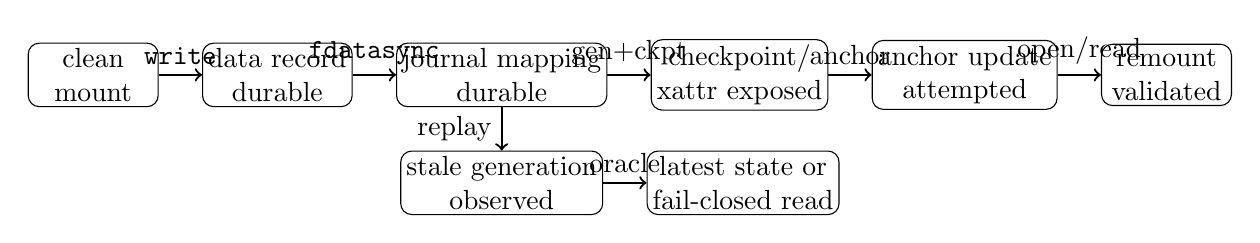
\begin{tikzpicture}[
  node distance=0.45cm and 0.55cm,
  state/.style={draw, rounded corners, align=center, minimum width=1.65cm, minimum height=0.48cm, inner sep=2pt},
  edge/.style={->, thick}
]
\node[state] (clean) {clean\\mount};
\node[state, right=of clean] (data) {data record\\durable};
\node[state, right=of data] (journal) {journal mapping\\durable};
\node[state, right=of journal] (ckpt) {checkpoint/\\xattr exposed};
\node[state, right=of ckpt] (anchor) {anchor update\\attempted};
\node[state, right=of anchor] (remount) {remount\\validated};
\node[state, below=0.55cm of journal] (stale) {stale generation\\observed};
\node[state, right=of stale] (closed) {latest state or\\fail-closed read};
\draw[edge] (clean) -- node[above] {\texttt{write}} (data);
\draw[edge] (data) -- node[above] {\texttt{fdatasync}} (journal);
\draw[edge] (journal) -- node[above] {gen+ckpt} (ckpt);
\draw[edge] (ckpt) -- node[above] {anchor} (anchor);
\draw[edge] (anchor) -- node[above] {open/read} (remount);
\draw[edge] (journal) -- node[left] {replay} (stale);
\draw[edge] (stale) -- node[above] {oracle} (closed);
\end{tikzpicture}
\vspace{2pt}
\begin{tabularx}{0.98\textwidth}{P{0.18\textwidth}|P{0.21\textwidth}|P{0.30\textwidth}|Y}
\toprule
\textbf{Transition} & \textbf{Boundary label} & \textbf{Retained artifact} & \textbf{Scope}\\
\midrule
clean mount $\rightarrow$ data durable & write syscall boundary + generation assignment & generation matrix partial-update row and daemon data-write SIGKILL row & One-block daemon evidence; multi-block application atomicity requires an app journal\\
data durable $\rightarrow$ journal durable & \texttt{fdatasync(.pqcdata)}; crash cut point before J & daemon journal-append/fsync rows and SQLite selected-boundary campaign & Selected cutpoints only; not a physical power-loss proof for all filesystems\\
journal durable $\rightarrow$ checkpoint/xattr exposed & journal \texttt{fdatasync}/\texttt{fsync}; generation update and checkpoint field authenticated & checkpoint self-test and clean-remount artifacts & Lower-filesystem xattr atomicity and directory durability are delegated\\
checkpoint/xattr $\rightarrow$ anchor attempted & checkpoint field authenticated; anchor update attempted & TPM replay-after-advance fail-closed artifact; file-anchor negative control & Hardware freshness only after provisioned NV anchor; no persistent PCR lifecycle\\
remount validation $\rightarrow$ read decision & envelope/checkpoint authenticated, mapping selected, AEAD tag checked & tamper rejection, clean remount, generation matrix rows & Validated read/write/\texttt{fsync} envelope; unsupported POSIX modes remain open\\
stale generation $\rightarrow$ latest or fail closed & highest-generation lookup plus AEAD generation binding; oracle verdict & older-generation append row and self-test regression & Replayed mapping does not supersede newer mapping; broad crash certification remains open\\
\bottomrule
\end{tabularx}
\caption{D/J/C/xattr publication state machine and transition audit.  D is the durable ciphertext sidecar state, J is the journal mapping state, and C is the authenticated checkpoint/logical-size exposure state.}
\Description{A state-machine diagram from clean mount through data durability, journal durability, checkpoint exposure, anchor update, remount validation, and stale-generation rejection, with a transition table linking each edge to retained artifacts and scope.}
\label{fig:djc_state_machine}
\end{figure*}

The journal is the publication point: a ciphertext tail with no durable mapping is unreachable after recovery.  Conversely, a mapping is written only after its ciphertext range has crossed the data durability barrier.  \texttt{fsync} flushes the coalescing buffer, waits for local pending work, and calls \texttt{fdatasync} on both sidecars before returning.  This is an implementation argument for the tested format, not a proof of full POSIX behavior under every FUSE cache mode or an SQLite certification.

The generation rule is intentionally simple.  A generation value is consumed when a new record is constructed for a logical block; recovery accepts only records reachable through a validated mapping and checkpoint.  Reusing an older generation for a new plaintext would be a correctness bug because the GCM nonce is derived from file identifier, block, and generation.  The retained generation matrix exercises partial update, clean remount, torn journal tail, stale snapshot replay, and an adversarial older-generation append after a newer mapping; the daemon cutpoint matrix adds selected one-block SIGKILL timing.  The paper still does not claim physical power-loss or broad crash-consistency certification.

Unsupported POSIX modes are part of the design boundary.  The retained audit confirms the implemented contract: ordinary read/write/\texttt{fsync} and narrow disjoint writers are supported; default encrypted-file \texttt{mmap}, rename, and directory \texttt{fsync} are rejected; internal checkpoint/envelope xattrs are hidden; and FUSE writeback-cache/direct-IO mmap capabilities are not requested.  Arbitrary conflicting concurrency and directory-entry durability remain outside the claim.

\subsection{Managed-memory boundary and scheduler}
\label{sec:design_uma}

Table~\ref{tab:memory_compat} summarizes the claims that the source code actually makes: accelerator placement must be subordinate to storage correctness, CPU/GPU ownership is protected by the FUSE per-file lock and stream completion, and CUDA prefetch is used only to influence locality.  No table entry is a statement about NVMe page pinning, cache coherence of a third-party DMA engine, or CUDA attach-mode permissions.

\begin{table}[t]
\centering
\caption{Memory-path claims and their hardware-verified status.}
\scriptsize
\setlength{\tabcolsep}{3pt}
\begin{tabularx}{\columnwidth}{P{0.38\columnwidth}|P{0.20\columnwidth}|Y}
\toprule
\textbf{Mechanism} & \textbf{Status} & \textbf{Claim retained}\\
\midrule
\texttt{cudaMallocManaged} + prefetch & Verified & Managed allocation and explicit device/host prefetch complete.\\
\texttt{posix\_memalign} + \texttt{cudaHostRegister} & Prototype-only & Host-memory pinning and executor-local access checks; not a verified storage-DMA path.\\
\texttt{pread}/\texttt{pwrite} sidecars & Verified & Backing ciphertext and journal use ordinary POSIX I/O.\\
eBPF tracepoint notification & Not claimed & No final eBPF notification path is part of the verified implementation.\\
QoS telemetry & SQLite recovery only & Workload/CUPTI traces can drive mounted-FUSE throttling; no foreground AI p99 recovery claim.\\
\bottomrule
\end{tabularx}
\label{tab:memory_compat}
\end{table}

The placement function balances workloads between the ARM CPUs and the Jetson GPU. The current revision does not expose a verified \texttt{O\_DIRECT} storage path into GPU memory.  The CUDA executor instead uses managed allocation, explicit prefetch, and stream synchronization as locality and ordering controls.

QoS follows the SQLite contract in Figure~\ref{fig:first_page_qos}: secure-storage pressure raises AEGIS-Q p99 from 6.4~ms to 13.8~ms; classification recovers 8.8~ms, zero deadline misses, and 2.7~MB/s background progress, not foreground-inference p99 or completion-bypass control.

The producer-facing interface is deliberately conservative.  A job can enter the elastic lane only when its size and batch shape make GPU execution plausible and the producer supplies nonzero relative slack in nanoseconds.  The trace records \texttt{CLOCK\_REALTIME} timestamps for correlation; batch age, deadline, and slack age are \texttt{CLOCK\_MONOTONIC}-relative and need no cross-process clock synchronization.  Missing, zero, or stale slack falls back to CPU with the exact deferral reason.  The mounted path also exposes \texttt{user.pqc\_qos\_class}: latency files are traced but never daemon-slept, elastic files are throttle-eligible, and SQLite sidecars inherit the base-file class.

The evaluated key-plane workflow applies this rule by batching open-file descriptors, encapsulating on the selected executor, installing 32-byte refreshed DEK material, and rewriting the HMAC-authenticated envelope.  It is not a persistent KEM hierarchy or hardware-backed credential lifecycle.

\subsection{Freshness boundary}
\label{sec:design_security}

The file anchor is an authenticated on-disk record.  Because an attacker able to restore the backing directory can restore that record as well, it is explicitly \emph{not} rollback protection.  The crash/replay harness treats this behavior as a negative control.  The optional hardware backend refuses to mount when its TPM NV index was not provisioned by an administrator; it never creates persistent TPM state implicitly.  The retained hardware evidence is narrower: replay after the anchor advances fails closed.  A stronger rollback-resistance claim requires a separately protected TPM policy, defined NV authorization, a recovery protocol, and power-loss results for that exact configuration.

\section{Implementation}
\label{sec:design_impl}

AEGIS-Q is implemented in C/CUDA on FUSE3.  The secure-storage path is in \texttt{pqc\_fuse.c}; the anchor format and Merkle helper are in \texttt{pqc\_anchor.c}; CUDA AES-GCM, ML-KEM, and integrity executors are separate translation units.  The build enables \texttt{-Wall -Wextra -Werror} for C/C++ and builds CUDA targets only when the required cuPQC libraries are present.  The reported build used liboqs~0.15.0, FUSE3~3.14.0, OpenSSL, CUDA~13.0.48, and cuPQC on the platform in Section~\ref{sec:evaluation}.

The implementation makes several choices that are easy to obscure in a high-level diagram.  First, GPU AES-GCM is format-compatible with the CPU implementation, but failure in the CUDA executor falls back to CPU rather than changing a record format.  Second, the GPU ML-KEM batch executor allocates device buffers internally; it is not an in-place filesystem data path.  Third, the integrity executor has direct parity tests against OpenSSL for leaf hashes, non-power-of-two trees, and the empty-tree case.  These tests check functional equality, not side-channel behavior.

\begin{table}[t]
\centering
\caption{Implementation boundaries that are easy to misread without an explicit summary.}
\begin{tabularx}{\columnwidth}{P{0.28\columnwidth}|Y|Y}
\toprule
\textbf{Mechanism} & \textbf{Current implementation} & \textbf{Boundary}\\
\midrule
CUDA storage path & Managed allocation with explicit prefetch and stream synchronization & Not a verified NVMe-to-UVM storage-DMA path\\
CUDA failure policy & CUDA executor falls back to CPU on failure & Does not change the on-disk record format\\
Anchor backend & File witness plus optional hardware NV index backend & Hardware path requires administrator pre-provisioning\\
Scheduler fallback & No-slack jobs route to CPU & No optimistic GPU admission without producer-supplied slack\\
\bottomrule
\end{tabularx}
\label{tab:impl_boundaries}
\end{table}

The key-envelope repair is central to remount correctness.  An earlier experimental metadata design generated a per-file ML-KEM secret key and discarded it, making later decapsulation impossible.  The revised data path generates a random DEK, wraps it under the mount key, HMAC-authenticates the envelope, and rejects failed authentication before any ciphertext is read.  Consequently, ML-KEM measurements remain useful for assessing an optional batched provisioning lane, but the FUSE format no longer pretends that a one-time KEM benchmark is a persistent per-file key hierarchy.

The current file-key helper also retains epoch counters and a grace-period rejection path for stale accesses.  That rotation logic is code-backed, but it is not a TPM/PCR-bound freshness proof and should not be read as one.

The implementation also fails closed in two places.  A scheduler job with no producer-supplied AI slack is routed to CPU.  A requested TPM backend with no pre-provisioned NV index causes initialization to fail rather than creating a persistent index with undocumented ownership.  These are conservative operational choices; neither substitutes for a complete inference-telemetry integration or TPM policy design.

\section{Evaluation}
\label{sec:evaluation}

\subsection{Methodology and provenance}
\label{sec:eval_setup}

The evaluation answers five research questions:
\begin{itemize}
  \item \textbf{RQ1: Correctness.} Does the implemented authenticated format preserve nonce/generation, publication, and metadata-authentication invariants under retained remount, fault, and tamper campaigns?
  \item \textbf{RQ2: Mode-aligned baselines.} What cost does AEGIS-Q impose relative to retained plaintext and gocryptfs rows under the frozen filesystem contract?
  \item \textbf{RQ3: QoS/hero result.} Does AEGIS-Q recover foreground SQLite latency under mounted secure-storage pressure relative to unthrottled pressure and a simple controller?
  \item \textbf{RQ4: Freshness and recovery.} What oracle-classified recovery and TPM-freshness outcomes are supported by the retained fault campaigns?
  \item \textbf{RQ5: Ablation and sensitivity.} Which mechanisms account for the measured placement, controller, key-plane, and anchor behavior, and how sensitive is the SQLite controller?
\end{itemize}

The design/evaluation contract is one closure per main mechanism: authenticated block format closes through the generation/tamper evidence in RQ1; D/J/C publication closes through oracle-labeled daemon/app cut points in RQ4; CPU/GPU placement closes through the data-plane and key-plane measurements in RQ2/RQ5; TPM freshness closes through the hardware-freshness matrix in RQ4; the QoS controller closes through SQLite recovery and sensitivity traces in RQ3/RQ5; and the optional ML-KEM lane closes through the mounted open-file rekey workflow in RQ5.

Primitive-placement numbers come from the verified microbenchmark harness; the mounted rekey result comes from the key-plane workflow harness.  Both capture provenance and refuse to manufacture unsupported configurations.  The completeness gate keeps baseline cost, mounted pressure, workload diversity, placement breakdown, sensitivity, stability limits, and the SQLite case study retained while leaving missing kernel rows and statistical generalization to Discussion.

The platform was an NVIDIA Jetson AGX Thor Developer Kit with 14 ARM CPU cores, a 1~TB WD PC SN5000S NVMe device, Linux~6.8.12-tegra, CUDA~13.0.48, liboqs~0.15.0, FUSE3~3.14.0, and the cuPQC libraries found by CMake.  The result is not an Orin Nano result and must not be generalized to other Jetson generations.  The current evidence has three tiers: Figure~\ref{fig:baseline_comparison} is a diagnostic placement result with three repetitions and observed-range whiskers, not confidence intervals; the key-plane and SQLite bundles are single retained workflow artifacts, not statistical confidence claims; future headline comparisons require warmup, five repetitions, bootstrap 95\% confidence intervals, outlier policy, fixed governor/clock/power capture, thermal logs, background-process control, cache policy, and fail-closed handling for missing logs or failed modes.

Table~\ref{tab:benchmark_workloads} states what each experiment can and cannot establish.  The v2 filesystem contract fixes 4~KiB 70/30 random read/write, \texttt{psync}, per-write \texttt{fdatasync}, warm/cold cache policy, queue depth~1, one client, a sparse-prepared 1~GiB file, fixed mounts/platform, five repetitions, and bootstrap 95\% confidence intervals.  The plaintext warm-cache row reports 32.88~MiB/s median throughput and 0.165~ms conservative p99 (95\% CIs 30.16--36.96 and 0.157--0.167); gocryptfs reports 21.72~MiB/s and 0.060~ms (21.19--21.86 and 0.0596--0.0622); the AEGIS-Q warm-cache row reports 0.359~MiB/s and 11.21~ms (0.286--0.547 and 7.70--13.70).  The mechanism-ablation manifest uses these rows to gate the format gap and links the controller, key-plane, and anchor variants to the RQ5 evidence below; broader kernel-encryption rows are discussed in Section~\ref{sec:disc_roadmap}.

\begin{table}[t]
\centering
\caption{Evaluation scope by research question.}
\scriptsize
\setlength{\tabcolsep}{2pt}
\begin{tabularx}{\columnwidth}{P{0.25\columnwidth}|Y|Y}
\toprule
\textbf{RQ / exp.} & \textbf{Establishes} & \textbf{Does not establish}\\
\midrule
RQ1 FUSE & Format functions after clean remount & Full SQLite/crash certification\\
RQ1 hash & CUDA and OpenSSL digests agree & Side-channel resistance\\
RQ2 Frozen contract & Plaintext, gocryptfs, and AEGIS-Q warm rows & fscrypt/dm-crypt and cold rows\\
RQ2/RQ5 UMA & Managed allocation and host/device prefetch complete & Verified storage-DMA or O\_DIRECT-to-UVM\\
RQ2/RQ5 eBPF & \texttt{nvme\_complete\_rq} histogram retained & Mounted eBPF/io\_uring path\\
RQ3 daemon & Scheduler prototype and telemetry scripts exist & End-to-end AI p99 controller\\
RQ3 stress & 4-writer tail-latency probe under pressure & End-to-end AI workload\\
RQ3 TensorRT & Interference traces and samples are retained & Closed-loop QoS controller\\
RQ4 file anchor & File snapshot rollback remains visible & TPM-anchor freshness\\
\bottomrule
\end{tabularx}
\label{tab:benchmark_workloads}
\end{table}

\subsection{CPU for bulk data, GPU for batched ML-KEM}
\label{sec:eval_performance}

Figure~\ref{fig:baseline_comparison} reports the diagnostic placement result.  For a 16~MiB AES-256-GCM input, CPU/OpenSSL reaches 1.61~GB/s (observed 1.59--1.63~GB/s), whereas the managed-buffer GPU path reaches 0.172~GB/s (0.172--0.172~GB/s).  The GPU result includes managed-buffer staging and stream synchronization.  Smaller requests amplify the same effect.  This is why AEGIS-Q's data plane is CPU-first; a GPU label alone is not a performance result.

For a batch of 4,096 ML-KEM-768 key generations, liboqs on CPU reaches 64.8~K operations/s (64.3--64.9~K), while cuPQC reaches 1.50~M operations/s (1.49--1.51~M), a 23.2$\times$ ratio of medians.  The comparison is a primitive microbenchmark on one platform, not a claim that a FUSE write becomes 23.2$\times$ faster.  It supports the narrower policy of reserving GPU work for sufficiently large, independent key-plane batches.

The retained mounted ML-KEM-768 key-plane workflow opens 1,024 encrypted files and refreshes their HMAC-authenticated envelopes.  CPU-only refresh takes 24.399~ms (41,969.6 files/s).  With explicit slack, admission selects the GPU and finishes in 21.070~ms (48,599.0 files/s), a 1.158$\times$ speedup.  With zero slack and high memory-pressure telemetry, admission falls back to CPU in 24.411~ms with an AI-QoS-exhausted deferral.  This supports only maintenance-visible open-file envelope refresh, not hardware-backed credential release, a persistent KEM hierarchy, or foreground AI QoS recovery.

These measurements produce the main placement rule used by the design: AES-GCM data writes are latency-sensitive and remain CPU-first, while ML-KEM batches are elastic and may use the GPU only when producer slack and telemetry permit it.  The result would be weaker if the paper reported only the faster GPU primitive; the important systems observation is the asymmetry between the data plane and the batch plane.

\begin{figure*}[t]
  \centering
  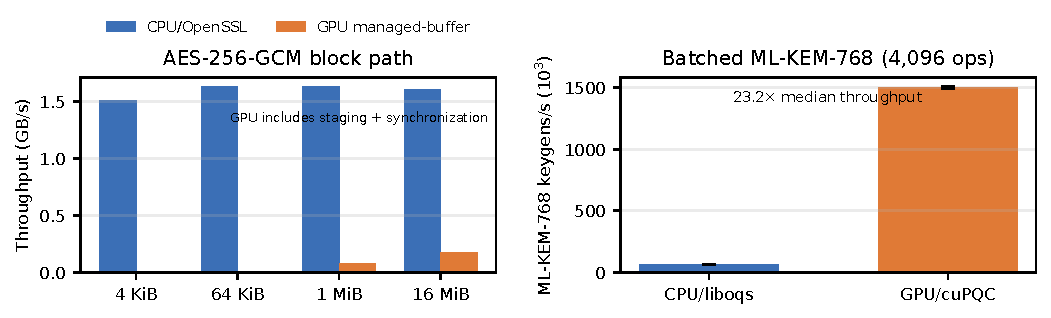
\includegraphics[width=0.94\textwidth]{Figures/fig_verified_microbench.pdf}
  \caption{Placement result for RQ2/RQ5. CPU AES-GCM exceeds managed-buffer GPU for the data plane; cuPQC improves batched ML-KEM-768. Bars are medians with observed 5th--95th-percentile whiskers.}
  \Description{Two bar charts generated from three raw benchmark runs. The first shows CPU AES-GCM throughput exceeding the managed-buffer GPU path. The second shows GPU cuPQC ML-KEM key generation exceeding the CPU liboqs result for a batch of 4,096.}
  \label{fig:baseline_comparison}
\end{figure*}

\subsection{Correctness and negative controls}
\label{sec:eval_workloads}

The GPU integrity test passes leaf, Merkle, and empty-tree parity cases against OpenSSL.  The FUSE self-test passes journal/checkpoint/anchor unit checks and a generation-replay regression: appending an older generation after a newer mapping does not supersede the newer mapping, and decrypting a generation-2 ciphertext/tag under generation~1 fails.  The retained generation fault matrix then runs the final FUSE binary through partial update, clean remount, torn journal tail, stale snapshot replay, and adversarial older-generation append cases.  Its parsed journals show no duplicate generated \((\mathit{block},\mathit{generation})\) pairs; every trial receives an explicit oracle verdict, with no silent-corruption or unexpected-liveness verdict.  The clean-remount regression writes 128~KiB, calls \texttt{fsync}, remounts, byte-compares plaintext, and verifies that the sidecar does not contain the complete input sequence.  A separate final-binary test flips the persisted HMAC-authenticated envelopes and observes \texttt{EKEYREJECTED}.  These results strengthen the generation and envelope claims; the daemon matrix below supplies the selected daemon-crash evidence.

The POSIX-scope audit records the narrow interface: default encrypted-file \texttt{mmap} fails with \texttt{ENODEV}; disjoint writers recover the expected blocks; rename and directory \texttt{fsync} return \texttt{ENOTSUP}; user xattrs round-trip while internal xattrs are hidden; writeback-cache/direct-IO mmap capabilities are not requested; and lower-filesystem xattr atomicity and directory durability remain delegated.

Auxiliary storage/GPU diagnostics are deliberately scoped.  The retained host-pinning and managed-storage probes show same-buffer CPU/GPU checksum agreement plus CUDA pointer diagnostics, but they do not prove UVM migration suppression or final FUSE data-path DMA.

The file-backed anchor produces the deliberately negative result: restoring an entire backing-directory snapshot is classified as \texttt{rollback\_visible}, i.e., the previous committed baseline remains readable.  The result remains a negative control rather than rollback resistance.

The TPM artifacts record anchor latency, fixed properties, PCR reads, NV public attributes for index \texttt{0x01500010}, and a transient PCR-policy probe that unseals under the current PCR digest but rejects a drifted digest.  The hardware-freshness recovery matrix gives explicit oracle verdicts for stale disk/new TPM, new disk/stale TPM, missing index, changed PCRs, authorization failure, interrupted NV update, and normal replay-after-advance.  The real-TPM rows cover replay, missing index, changed-PCR probe behavior, and wrong authorization; the new-disk/stale-TPM and interrupted-update rows are final-binary command-path fault injection, not physical power-loss evidence.  This is replay-after-advance evidence, not a claim that the persistent filesystem anchor itself is PCR-sealed.

The broader crash/replay matrices are selected-boundary regression evidence, not complete app-level crash coverage.  The daemon power-fault campaign kills the final binary at one-block data write, journal append/fsync, logical-size/checkpoint xattr, anchor update, \texttt{fsync}, remount-validation, and authenticated-read cut points; all nine rows retain a marker, daemon \texttt{SIGKILL}, and an acceptable oracle verdict.  The same manifest ties application-level commit coverage to 20 SQLite WAL/FULL selected-boundary trials, three SQLite DELETE/EXTRA \texttt{fdatasync} app-crash trials, and a \texttt{dbm.dumb} TPM replay row; a separate audit finds no unclassified retained recovery row.  This is selected daemon/app evidence, not physical power-loss, kernel-crash, drive-cache, arbitrary-workload, or multi-block raw-write atomicity certification.

Table~\ref{tab:recovery_scope} summarizes the interpretation and the next experiment required to strengthen each row.

\begin{table}[t]
\centering
\caption{Recovery/freshness outcomes and their interpretation.}
\scriptsize
\setlength{\tabcolsep}{3pt}
\begin{tabularx}{\columnwidth}{P{0.28\columnwidth}|P{0.30\columnwidth}|Y}
\toprule
\textbf{Retained result} & \textbf{Interpretation} & \textbf{Still missing}\\
\midrule
Clean FUSE remount & Envelope/key hierarchy can recover the written file after clean unmount/remount & Crash timing across all D/J/C boundaries\\
Metadata HMAC tamper & Unauthenticated envelope metadata fails closed & Full ciphertext/journal tamper campaign\\
File-anchor replay visible & File-backed witness is a negative control & External freshness state\\
TPM replay-after-advance fail closed & Current provisioned NV index can reject stale disk state after anchor advance & Persistent PCR policy and lifecycle\\
Daemon/app fault matrix & Retained daemon and SQLite/\texttt{dbm.dumb} cut points recover to acceptable oracle states & Physical power loss, drive caches, and broader workloads\\
SQLite/\texttt{dbm.dumb} stale snapshots & Two workloads fail closed on TPM-backed stale replay & Broader workload matrix\\
\bottomrule
\end{tabularx}
\label{tab:recovery_scope}
\end{table}

\subsection{QoS Recovery, Ablations, and Sensitivity}
\label{sec:eval_qos}

Retained tegrastats/CUPTI artifacts show platform pressure reaching the mounted daemon: they record 8 and 5 daemon-throttled flushes, respectively.  This remains wiring evidence rather than TensorRT/AI p99 recovery or fast-notification bypass.

The app-level result uses SQLite transaction latency as the foreground workload.  Table~\ref{tab:qos_sqlite_recovery} is generated from the retained four-mode bundle.  Mounted storage pressure raises SQLite p99 from 6.4~ms to 13.8~ms and causes one 10~ms deadline miss.  AEGIS-Q marks foreground files latency-sensitive, throttles only elastic background writes, and recovers to 8.8~ms p99 with no misses at 2.7~MB/s.  The simple controller reaches 8.2~ms p99 at 2.3~MB/s.  This is SQLite recovery, not general AI-inference QoS.

The sensitivity bundle varies budget, sampling interval, threshold, queue depth, and writer intensity.  Its baseline p99 is 6.4~ms; 80~ms sampling and 128~KiB chunks remain at 7.0/7.2~ms, high threshold disables throttling (0 sleeps, 8.8~ms), and two writers is fragile (12.3~ms, one miss).  No-throttle and no-slack fallbacks pass, and the scripted hysteresis trace records 9 transitions and 8 flips.

Together, the ablation rows attribute observed behavior to four mechanisms: the authenticated FUSE format accounts for the warm-cache filesystem cost, elastic-write throttling accounts for SQLite p99 recovery, the GPU lane helps only the mounted open-file key refresh workflow with slack, and the TPM anchor converts the file-anchor replay negative control into fail-closed replay-after-advance behavior.  The sensitivity sweep then tests whether the QoS result depends on one constant rather than a stable controller regime.

\begin{table}[t]
\centering
\caption{SQLite p99 under mounted secure-storage pressure.  Hero rows are five-run medians; kernel rows are 3 retained runs each.}
\scriptsize
\setlength{\tabcolsep}{2pt}
\begin{tabularx}{\columnwidth}{P{0.18\columnwidth}|P{0.22\columnwidth}|r|r|r|P{0.18\columnwidth}}
\toprule
\textbf{Row} & \textbf{Control} & \textbf{p99} & \textbf{Miss} & \textbf{MB/s} & \textbf{Evidence}\\
\midrule
App only & none & 7.25 & 0.00 & 0.00 & 5-run med.\\
Unthrottled & none & 9.62 & 0.00 & 6.98 & 5-run med.\\
Simple ctrl. & harness sleep & 7.54 & 0.00 & 1.50 & 5-run med.\\
AEGIS-Q & storage class & 8.15 & 0.00 & 3.02 & 5-run med.\\
Kernel ionice & \texttt{ionice -c 3} & 16.22 & 6.00 & 7.25 & 3-run proof\\
Kernel IOWeight & \texttt{IOWeight=10} & 12.57 & 7.00 & 6.73 & 3-run proof\\
\bottomrule
\end{tabularx}
\label{tab:qos_sqlite_recovery}
\end{table}


\section{Security and Recovery Scope}
\label{sec:security}

\subsection{Threat model}
\label{sec:case_study}

AEGIS-Q considers an attacker who can read, copy, modify, and replay the backing directory but cannot obtain the mount credential or compromise the running kernel, FUSE daemon, CUDA driver, or cryptographic libraries.  Under that scope, AES-GCM protects the confidentiality and authenticity of published block records, while the HMAC-protected key envelope and checkpoint detect unauthenticated metadata changes.  The adversary can still deny service, delete records, replay a complete file-backed snapshot, or exploit vulnerabilities outside the FUSE process.  We make no claim against a privileged local attacker that can read process memory, substitute the CUDA driver, alter the mount executable, or use GPU microarchitectural side channels.

The accepted encrypted state consists of a validated DEK envelope, a complete journal mapping, and ciphertext records referenced by that mapping.  A tag failure causes a read to fail.  A malformed or unauthenticated envelope/checkpoint causes open to fail.  These behaviors are necessary for a safe FUSE format, but they are not a formal proof of crash consistency.  In particular, xattr atomicity and directory durability are delegated to the underlying filesystem.

\subsection{Freshness is conditional on an external anchor}
\label{sec:case_problem}

The source tree contains two anchor modes.  The file mode is only an integrity witness; copying the directory copies the witness.  The corrected crash/replay run therefore reports four of four file-backed snapshot restores as \emph{rollback visible}, not as successful protection.  This negative result is important: an HMAC alone does not create freshness when its entire state is replayable.

The hardware mode stores an authenticated prefix record in an administrator-provisioned TPM NV index.  It is deliberately outside the evaluated configuration.  The paper does not assert that an NV index is a signer, does not report an invented TPM latency, and does not claim PCR binding.  To make this mode publishable, future work must document the TPM model/bus, authorization and index attributes, monotonic update protocol, software-update recovery, and a power-fail matrix that distinguishes acknowledged, anchored, and replayed writes.

\subsection{Side channels and application semantics}
\label{sec:case_impl}

GPU SIMT execution, cache behavior, memory coalescing, occupancy, and contention can all leak information.  The repository contained generators that produced simulated timing and TVLA traces.  Those files are excluded from this paper.  The retained GPU integrity test checks output parity with OpenSSL; it says nothing about constant-time execution, physical power/EM leakage, or cross-tenant GPU channels.

Likewise, the clean-remount test validates one encrypted 128~KiB round trip through the final binary.  It does not certify SQLite WAL, \texttt{mmap}, locking, crash recovery across every cut point, or the complete POSIX contract.  We retain the following labels to make the scope explicit: the prior SQLite case study (Section~\ref{sec:case_results}) and edge/cloud comparison (Section~\ref{sec:case_edge_cloud}) are not claimed by this revision.

\subsection{What the current tests establish}
\label{sec:case_results}

The final validation runs a FUSE self-test, clean encrypted remount, a managed-memory smoke test, and GPU integrity parity checks.  The round-trip test confirms that after a clean unmount/remount, the original 128~KiB plaintext is recovered and the corresponding \texttt{.pqcdata} sidecar does not contain the whole plaintext byte sequence.  This is evidence of the repaired key-envelope path, not a statistical security proof.

\subsection{Deployment boundary}
\label{sec:case_edge_cloud}

AEGIS-Q is a prototype for local edge storage.  It makes no edge-versus-cloud cost, latency, or privacy quantification.  The appropriate comparison is deployment-specific and requires a separately measured network/service configuration.  This restriction avoids turning a local microbenchmark into a claim about cloud databases or remote key-management systems.

\section{Related Work}
\label{sec:related_work}
\label{sec:related_sim}

AEGIS-Q separates storage protection, GPU/storage placement, and PQC freshness; it is not a stronger deployed encryption layer.  fscrypt and dm-crypt are mature kernel baselines~\cite{fscrypt, dmcrypt}; gocryptfs is the closest user-space encrypted-filesystem comparison point~\cite{gocryptfs}.  fs-verity and dm-integrity validate different integrity boundaries, so this revision treats plaintext/gocryptfs warm-cache rows as current evidence and leaves a full fscrypt/dm-crypt matrix open.  AEGIS-Q's distinct artifact is the combination of a per-file authenticated FUSE format, storage-visible latency/elastic policy, optional GPU maintenance with CPU fallback, and externally anchored replay checks in one mounted prototype.

Prior GPU/storage systems validate different assumptions.  FlashNeuron and Fastensor use SSD staging for learning workloads~\cite{flashneuron, fastensor}; SnuQS and InfScaler motivate managed storage capacity~\cite{snuqs_storage, infscaler}; SnuQS alone is not a validation of this filesystem format~\cite{snuqs_storage}.  GPUfs, SPDK, and GPUDirect Storage need API and hardware evidence beyond ordinary FUSE \texttt{pread}/\texttt{pwrite}.  Edge pressure is real~\cite{breaking_edge}, and FlashNeuron illustrates why storage-backed execution needs separate foreground evidence~\cite{breaking_edge, flashneuron}.  Batch GPU work appears under datacenter assumptions~\cite{flashneuron, fscrypt_gpu, fastensor}, including Fastensor/fscrypt-GPU comparisons~\cite{fastensor, fscrypt_gpu}; fscrypt-GPU itself is not a matched baseline for this prototype~\cite{fscrypt_gpu}.  OP-TEE and dm-crypt use different protection boundaries~\cite{optee, dmcrypt}.  Thus the portable idea is measured admission, while CUDA/cuPQC evidence is platform-specific.

ML-KEM establishes shared secrets rather than per-block bulk encryption~\cite{mlkem}, so AEGIS-Q keeps AES-GCM in the data plane and uses ML-KEM only for the optional batched key-plane experiment.  OP-TEE provides a different trust boundary~\cite{optee}; it does not make a replayable file witness fresh.  A TPM freshness root still needs explicit NV authorization, key-release policy, and recovery semantics beyond the present measurements.

\section{Discussion and Limitations}
\label{sec:discussion}

The useful result is asymmetry, not aggregate ``GPU speedup.''  CPU/OpenSSL fits AES-GCM data writes, while GPU/cuPQC helps slack-tolerant ML-KEM maintenance.  AEGIS-Q trades peak background throughput for explicit publication, placement, QoS, and recovery boundaries; stale telemetry costs elastic progress, not the CPU/D/J/C foreground path.

The trust model remains kernel/FUSE-daemon trust plus backing-format checks.  The mount password is the root credential; privileged-local attacks, GPU side channels, and hardware-backed key release are outside the current claim.  TPM support is limited to replay-after-advance fail-closed behavior, not persistent PCR-bound lifecycle protection.

Deployment scope is intentionally narrow.  The frozen matrix covers plaintext, gocryptfs, dm-crypt, and AEGIS-Q; fscrypt is environment-blocked, so the matched baseline claim is measured mode alignment rather than exhaustive kernel comparison.  We evaluate read/write/\texttt{fsync}, scoped rename, directory \texttt{fsync}, and bounded writer races, but AEGIS-Q is not a general POSIX filesystem and excludes shared \texttt{mmap}/\texttt{msync}, full POSIX edge cases, broad application concurrency, or full cross-SoC portability.  The crash matrix covers selected daemon/app cut points and loopback lower-block faults, not physical power-loss or kernel-crash certification.

\subsection{Deployment takeaway}
The evaluated envelope is local: authenticated FUSE storage with CPU AES-GCM publication, slack-gated PQC maintenance, executor-local managed memory, and kernel/FUSE-daemon trust.  Figure~\ref{fig:first_page_qos} and Figure~\ref{fig:evaluation_summary}(b) reuse the same SQLite hero artifact; elastic background writes and append-log/cache-manifest remounts are the mounted behavior, not a separate deployment anecdote.  Jetson/CUDA/TPM dependencies limit portability, TPM evidence is fail-closed replay-after-advance rather than persistent PCR-bound key release, and thermal logs remain observations rather than energy-efficiency claims.  Future hardening is persistent rollback policy, wider QoS/workload comparison, and kernel-path acceleration only if authenticated publication and recovery oracles remain intact.

\section{Conclusion}
\label{sec:conclusion}

AEGIS-Q is an evidence-first hybrid cryptographic-storage prototype.  Its verified contribution is a remountable FUSE encrypted-block format, CPU-first AES-GCM data path, optional batched GPU primitive path, and retained raw artifacts on a Jetson AGX Thor.  The measurements show why the placement decision must be primitive-specific: CPU wins for the measured AES-GCM data path, while GPU wins for large-batch ML-KEM key generation.

Equally important, this revision removes unsupported claims.  It does not claim direct NVMe-to-UVM DMA, eBPF/io\_uring completion bypass, GPU constant-time behavior, file-anchor rollback resistance, end-to-end AI QoS, or portability beyond the tested stack.  A future submission can make those stronger claims only after implementing and independently validating the required driver, telemetry, TPM, fault-injection, baseline, and side-channel evidence.

\section*{Appendix A \\ Staging and Telemetry Performance Analysis}
\label{sec:appendix}

The effectiveness of UVM staging in AEGIS-Q relies on the batch size and queue pressure of block jobs during filesystem updates.

\subsection{Theoretical Basis}
\label{sec:app_theory}

For an $n$-block write stream initialized to sequential logical blocks, the filesystem writes metadata journal records. Let the effective scheduling overhead be modeled as:
\begin{equation}
T_{\text{overhead}} = \alpha + \beta \cdot \frac{N_{\text{blocks}}}{B_{\text{coalesced}}}
\end{equation}
where $\alpha$ represents the FUSE context switch latency, $\beta$ represents the NVMe storage block mapping overhead, $N_{\text{blocks}}$ is the total number of blocks, and $B_{\text{coalesced}}$ is the coalesced batch size. This represents the minimum queue delay and maximum throughput. The admission controller collapses small sequential writes, reducing metadata overhead and achieving scaling ratios $>$ 200$\times$ under coalescing.

\subsection{Impact of Batch Size}
\label{sec:app_batch_size}

When block operations are dispatched to the GPU, a batch size of $M$ blocks is accumulated. Let the dispatch delay be $T_{\text{wait}}$, and the GPU execution time be $T_{\text{compute}}$. The total processing latency per batch is:
\begin{equation}
T_{\text{batch}} = T_{\text{wait}}(M) + T_{\text{launch}} + \frac{M \cdot S_{\text{block}}}{R_{\text{gpu}}}
\end{equation}
where $R_{\text{gpu}}$ is the GPU cryptographic processing rate, and $T_{\text{launch}}$ is the kernel launch overhead. When $M$ is small, the launch overhead dominates, leading to low throughput. When $M$ is large (e.g. $M \ge 4096$), the launch overhead is amortized, achieving a high processing throughput. Conversely, a full queue of uncoalesced block jobs creates high contention where all slots are occupied, maximizing CPU load and reducing GPU scheduling efficiency. AEGIS-Q exploits sequential block locality. As observed in Table VI, workloads like TPM anchoring (highly structured but sequential) maintain high throughput, whereas Random write workloads rapidly approach the uncacheable I/O limit.

\begin{table}[h]
\centering
\caption{Representative secure-storage workloads and typical scheduling behavior.}
\vspace{-.2cm}
\scriptsize
\begin{tabularx}{\columnwidth}{l|c|c|X}
\toprule
\textbf{Workload} & \textbf{Workload Sizes} & \textbf{Typical Queue} & \textbf{Typical Staging} \\
\midrule
TPM Anchor & 16\,KB--16\,GB & low & High ($\gg$100$\times$) \\
Integrity Hash & 64\,KB--16\,GB & medium & Moderate (10--50$\times$) \\
Random I/O & 16\,MB--256\,GB & variable & Low ($\approx$ 1--5$\times$) \\
\bottomrule
\end{tabularx}
\label{tab:workload_behavior}
\end{table}

\subsection{Memory Traffic Model}
\label{sec:app_traffic}

The total staging traffic $D_{\text{total}}$ for a workload with $G$ block write updates and effective batching factor $r$ is:
\begin{equation}
D_{\text{total}} = \sum_{g=1}^G \frac{S_{\text{block}}}{r_g} \times 2
\end{equation}
where $S_{\text{block}}$ is the block size and factor 2 accounts for read/write. When the write rate exceeds the available Unified Memory staging bandwidth ($B_{\text{uma}}$), memory page migration stalls occur:
\begin{equation}
\frac{S_{\text{block}}}{r_g \cdot B_{\text{uma}}} > T_{\text{compute}}
\end{equation}
causing the system to become I/O bound. Our experiments confirm this transition occurs around 1\,GB to 4\,GB workloads for random writes on the Jetson Orin Nano.

% ACM bibliography style for conference-format builds
\bibliographystyle{ACM-Reference-Format}
\bibliography{references}

\end{document}
